\documentclass{article}
%Packages being imported that add functionality to LaTeX.
\usepackage[utf8]{inputenc}
\usepackage{geometry}
\usepackage{amssymb,amsmath,amsthm,mathtools,bussproofs,turnstile}
\usepackage{enumerate}
\usepackage{listings}
\usepackage{../common/vaucanson-g/vaucanson-g}
\usepackage{float}
\usepackage{epstopdf}
\usepackage{mathtools,array}
\usepackage[all]{xy}
\SelectTips{cm}{10}     % Use the arrowheads that agree with inline arrows.
\everyxy={<2.5em,0em>:}
%Theorem Environments
\newtheorem{theorem}{Theorem}[section]
\newtheorem{lemma}[theorem]{Lemma}
\theoremstyle{definition}
\newtheorem{definition}{Definition}[section]
\newtheorem{corollary}[theorem]{Corollary}


%valuations
\newcommand{\valuations}{\ensuremath{\mathbb{V}}}
\newcommand{\propositions}{\ensuremath{\mathbb{P}}\xspace}
\newcommand{\proposition}{\ensuremath{p}\xspace}
%\newcommand{\acceptingState}{acc}
%\newcommand{\acceptingSymbol}{\alpha}
%\newcommand{\acceptingSymbols}{\beta}
\newcommand{\executionDef}{\ensuremath{\varepsilon=s_0, \actionLabel_0, s_1, \ldots}\xspace}
\newcommand{\execution}{\ensuremath{\varepsilon}\xspace}

%clts
\newcommand{\cltsDefIdx}[1]{\ensuremath{#1 = \lparen S_{#1},} \ensuremath{\Sigma_{#1}, \Delta_{#1},} \ensuremath{s_{0}^{#1}, \propositions_{#1}, \valuations_{#1}\rparen}\xspace}
\newcommand{\cltsDefShareSigmaIdx}[1]{\ensuremath{#1 = \lparen S_{#1},} \ensuremath{\Sigma, \Delta_{#1},} \ensuremath{s_{0}^{#1}, \propositions_{#1},} \ensuremath{\valuations_{#1}\rparen}\xspace}
\newcommand{\cltsDef}{\ensuremath{E = (S, \Sigma, \Delta, s_{0}, \propositions, \valuations)}\xspace}
\newcommand{\cltsEmbeddingDef}[1]{\ensuremath{clts(#1) = (S, \Sigma, \Delta, s_{0}, \valuations)}\xspace}
\newcommand{\automaton}[1]{\ensuremath{#1 = (S_{#1}, \Sigma_{#1}, \Delta_{#1}, s_{0}^{#1})}\xspace}
\newcommand{\labelSet}{\ensuremath{\mathcal{L}}\xspace}
\newcommand{\actionLabel}{\ensuremath{L}\xspace}
\newcommand{\action}{\ensuremath{l}\xspace}
\newcommand{\traces}{\ensuremath{\emph{Tr}}}

%composition
\newcommand{\cltsComposition}[3]{{\ensuremath{#1 \parallel_{#3} #2 = \lparen S,$ $\Sigma_{#1} \cup \Sigma_{#2},$ $\Delta,$ $(s_{0}^{#1},s_{0}^{#2}),$ $\propositions_{#1} \cup \propositions_{#2}$ $\valuations\rparen}}\xspace}
\newcommand{\ltsAdjustment}[2]{{\ensuremath{#1 \pm #2 = \lparen S_{#1}\times S_{#2},$ $\Sigma_{#1} \cup \Sigma_{#2},$ $\Delta,$ $(s_{0}^{#1},$ $s_{0}^{#2})\rparen}}\xspace}

%control problem
\newcommand{\controlSet}{\ensuremath{\mathcal{C}}}
\newcommand{\nonControlSet}{\ensuremath{\mathcal{U}}}
\newcommand{\controlProblemDef}{\ensuremath{\controlProblem =\langle E,$ $\controlSet,$ $\varphi \rangle}\xspace}
\newcommand{\controlProblem}{\ensuremath{\mathcal{I}}}

%GS
\newcommand{\gsV}{{\ensuremath{\mathcal{V}}}\xspace}
\newcommand{\gsX}{{\ensuremath{\mathcal{X}}}\xspace}
\newcommand{\gsY}{{\ensuremath{\mathcal{Y}}}\xspace}
\newcommand{\gsTheE}{\ensuremath{{\theta_e}}\xspace}
\newcommand{\gsTheS}{\ensuremath{{\theta_s}}\xspace}
\newcommand{\gsRhoE}{\ensuremath{{\rho_e}}\xspace}
\newcommand{\gsRhoS}{\ensuremath{{\rho_s}}\xspace}

%FDS
\newcommand{\enumSet}[1]{\#(#1)}
\newcommand{\enumSetDef}{$\#:\mathcal{P}(\mathcal{M})\mapsto [0\ldots2^{|\mathcal{M}|}-1]$\xspace}
\newcommand{\fdsDefIdx}[1]{$#1= \langle \gsV_{#1},$ $\theta_{#1},$ $\rho_{#1},$ $\mathcal{J}_{#1},$ $\mathcal{C}_{#1}\rangle$\xspace}
\newcommand{\fdsD}{\ensuremath{\mathcal{D}}\xspace}
\newcommand{\fdsDef}{$\fdsD = \langle \gsV_d,$ $\theta_d,$ $\rho_d,$ $\mathcal{J}_d,$ $\mathcal{C}_d\rangle$\xspace}
\newcommand{\fdsControlProblemDef}{\ensuremath{\fdsControlProblem =\langle \gsX,} \ensuremath{\gsY,$ $\varphi \rangle}\xspace}
\newcommand{\fdsControlProblem}{\ensuremath{\mathcal{K}}\xspace}
%realizability theorems
\newcommand{\varState}[1]{\ensuremath{\hat{s}_{#1}}\xspace}
\newcommand{\varLabel}[1]{\ensuremath{\hat{l}_{#1}}\xspace}
\newcommand{\varphiLTL}{\ensuremath{\varphi_{FDS}}\xspace}
\newcommand{\varphiLTLDef}{\ensuremath{\varphiLTL = (\theta_e \implies \theta_s) \wedge (\theta_e \implies \square((\boxdot \rho_e) \implies \rho_s)) \wedge (\theta_e \wedge \rho_e \implies val(\varphi))}\xspace}
\newcommand{\varphiCLTS}{\ensuremath{\varphi_{CLTS}}}
\newcommand{\varphiCLTSDef}{\ensuremath{\varphiCLTS = ()}\xspace}
\newcommand{\varphiLtlFormula}{\ensuremath{(\theta_e \implies \theta_s) \wedge (\theta_e \implies \square((\boxdot \rho_e) \implies \rho_s)) \wedge (\theta_e \wedge \rho_e \implies val(\varphi))}}
\newcommand{\fdsEmbeddingDef}{\ensuremath{ltl(\controlProblem) = \langle \gsX,$ $\gsY,$ $\varphiLTL \rangle}\xspace}
\newcommand{\fdsEmbedding}{\ensuremath{ltl(\controlProblem)}\xspace}
\newcommand{\cltsCPEmbeddingDef}{\ensuremath{clts(\fdsControlProblem) =\langle E,$ $\controlSet,$ $\varphiCLTS \rangle}\xspace}
\newcommand{\cltsCPEmbedding}{\ensuremath{clts(\fdsControlProblem)}\xspace}


%formulae
\newcommand{\true}{\emph{true} }
\newcommand{\false}{\emph{false} }
\newcommand{\assume}{\phi}
\newcommand{\guarantee}{\gamma}
\newcommand{\invariant}{\rho}
\newcommand{\fluentp}[1]{\dot{#1}}
\newcommand{\fluent}{\emph{fl}}
\newcommand{\set}[1]{\{#1\}}
\newcommand{\gr}{{GR(1)}\xspace}
\newcommand{\sgr}{{SGR(1)}\xspace}
\newcommand{\G}{{\bf G}}
\newcommand{\F}{{\bf F}}
\newcommand{\X}{{\bf X}}
\newcommand{\U}{{\bf U}}


\title{Concurrent Labeled Transition Systems (CLTS)} %Change this to the appropriate number.
\author{Fundamentals} %Change this to your name.
\date{}

\begin{document}


\maketitle

%Counters for setting the appropriate numbering.
\setcounter{section}{1} %This gives the chapter number.
\setcounter{theorem}{1} %This gives the item number.
%Note that the item number should be one less than you desire..

\subsection{Concurrent Labeled Transition Systems (CLTS)}
\begin{definition}
	\actionLabel{def:CLTS} \emph{(Concurrent Labelled Transition Systems)} 
	A \emph{Concurrent Labelled Transition System} (CLTS) is defined as \cltsDef, where $S$ is a finite set of states, $\Sigma$ is its {\em set of actions}, $\Delta \subseteq (S \times 2^{|\Sigma|} \times S)$ is a transition relation, $s_0 \in S$ is the initial state, $\propositions : \{\proposition_0,\ldots,\proposition_k\}$ is a finite set of atomic propositions and $\valuations : S \mapsto  2^{|\propositions|}$ is the function that defines the set of propositions ¨that hold at a given state $s \in S$.  
	%We denote $\Delta(s)=\{\actionLabel~|~(s,\actionLabel,s') \in \Delta\}$. 
	A CLTS is deterministic if $(s,\actionLabel,s')$ and $(s,\actionLabel,s'')$ are in $\Delta$ then $s'=s''$ should hold.
	An execution of $E$ is a word \executionDef where $(s_i, \actionLabel_i, s_{i+1}) \in \Delta$. 
	%A word $\pi$ is a trace (induced by $\varepsilon$) of $E$ if its the result of removing every $s_i$ from an execution $\varepsilon$ of $E$. 	We denote the set of infinite traces of $E$ by $\traces(E)$. 
	Given a transition $(s_i, \actionLabel, s_j) \in \Delta$, we will call $\actionLabel$ its label, and each element $\action \in \actionLabel$ an action.
\end{definition}

\subsection{CLTS fluent satisfaction}

We use linear temporal logics of fluents (FLTL) over CLTS models. %~\cite{DBLP:conf/sigsoft/GiannakopoulouM03}. 
A \emph{fluent} \emph{fl} is defined by a pair of sets and a Boolean value: $\emph{\fluent} = \langle I_{\emph{\fluent}}, T_{\emph{\fluent}}, \emph{Init}_{\emph{\fluent}} \rangle$, where $I_{\emph{\fluent}}\subseteq \mathcal{P}(Act)$ is the set of initiating actions, $T_{\emph{\fluent}} \mathcal{P}(Act)$ is the set of terminating actions and $I_{\emph{\fluent}}\cap T_{\emph{\fluent}}=\emptyset$. 
A fluent may be initially \true or \false as indicated by \emph{Init}$_{\emph{\fluent}}$. 
Every actions $\ell\in Act$ induces a fluent, namely $\fluentp{\ell}=\langle \{\ell\}, \{Act\setminus \set{\ell}\}, \false\rangle$. 
Finally, the alphabet of a fluent is the union of its terminating and initiating actions.

Let $\mathcal{F}$ be the set of all possible fluents over $\mathcal{P}(Act)$. 
An FLTL formula is defined inductively using the standard Boolean connectives and temporal operators $X$~(next), $U$ (strong until) as follows: 
$\varphi ::= \fluent \mid \neg \varphi \mid \varphi \vee \psi \mid \X \varphi \mid \varphi U \psi,$
where $\fluent\in\mathcal{F}$. 
As usual we introduce $\wedge$, $\F$ (eventually), and $\G$ (always) as syntactic sugar. 
Let $\Pi$ be the set of infinite traces over \emph{Act}.
The trace $\pi=\ell_0,\ell_1,\ldots$ satisfies a fluent $\emph{Fl}$ at position $i$, denoted $\pi,i \models \emph{Fl}$, if and only if one of the following conditions holds:
\begin{list}{-}%{\leftmargin=3em}
	\item $\emph{Init}_{\emph{Fl}} \wedge (\forall j \in \mathbb{N} \cdot 0 \leq j \leq i \rightarrow \nexists t \in T_{\fluent}: t \subseteq \ell_j)$
	\item $\exists j \in \mathbb{N} \cdot (j \leq i \wedge \exists i \in I_{\fluent}: i \subseteq \ell_j) \wedge (\forall k \in \mathbb{N} \cdot j < k \leq i \ \rightarrow \nexists t \in T_{\fluent}: t \subseteq \ell_k)$
\end{list}

Given an infinite trace $\pi$, the satisfaction of a formula $\varphi$ at position $i$, denoted $\pi,i\models\varphi$, is defined as follows:

\begin{tabular}{ l c l }
$\pi, i \models_d \neg \varphi$ & $\triangleq$ & $\pi, i \not\models_d \varphi$\\
$\pi, i \models_d \varphi \vee \psi$ & $\triangleq$ & $(\pi, i \models_d \varphi) \vee (\pi, i \models_d \psi)$\\
$\pi, i \models_d \X \varphi$ & $\triangleq$ & $\pi, i +1 \models_d \varphi$\\
$\pi, i \models_d \varphi \U \psi$ & $\triangleq$ & $\exists j \geq i . \pi,j \models_d \psi \wedge \forall i \leq k \le k. \pi, k \models_d \varphi$\\
\end{tabular}
  
We say that $\varphi$ holds in $\pi$, denoted $\pi\models\varphi$, if $\pi,0\models\varphi$. 
A formula $\varphi \in \mbox{FLTL}$ holds in an CLTS $E$ (denoted $E \models \varphi$) if it holds on every infinite trace produced by $E$.
A \emph{fluent} \fluent \space is defined by a set of initiating actions $I_{\fluent}$, a set of terminating actions $T_{\fluent}$, and an initial value \emph{Initially}$_{\fluent}$.

That is,
%\begin{equation*}
$ \fluent = \langle I_{\fluent}, T_{\fluent} \rangle_{\emph{initially}_{\fluent}} $, 
where 
$I_{\fluent},T_{\fluent} \subseteq \mathcal{P}(\emph{Act})$ 
and $I_{\fluent} \cap T_{\fluent} = \emptyset.$\\
%\end{equation*}
%A fluent may be initially \true or \false as indicated by the \emph{Initially}$_{\fluent}$ attribute,
%When we omit \emph{Initially}$_{\fluent}$, we assume the fluent is
%initially \emph{false}. We use $\fluentp{\ell}$ as short for the
%fluent defined as $\fluent = \langle \ell,
%\emph{Act}\setminus\set{\ell} \rangle$.
%Given the set of fluents $\Phi$, an FLTL formula is defined
%inductively using the standard boolean connectives and temporal
%operators $\mathbf{X}$ (next), $\mathbf{U}$ (strong until) as
%follows:\\
%%\begin{equation*}
%$\varphi ::= \fluent \mid \neg \varphi \mid \varphi \vee \psi \mid
%\mathbf{X} \varphi \mid \varphi \mathbf{U} \psi$,
%%\end{equation*}
%where $\fluent \in \Phi$.


\subsection{CLTS composition}

When having to compose concurrent systems we define three different semantics that can be applied pairwise. Synchronous semantic $A ||_s B$ (Figure~\ref{fig:synchronous_composition})captures the composition of two components that share a single synchronizing event (implicit), where all participants should be able to make progress concurrently. The main motivation being digital components sharing a single clock. 
Asynchronous semantic $A ||_a B$ (Figure~\ref{fig:asynchronous_composition}) captures the interleaving interpretation of concurrency as found in LTS systems. 

\begin{figure}[h]
		\centering
	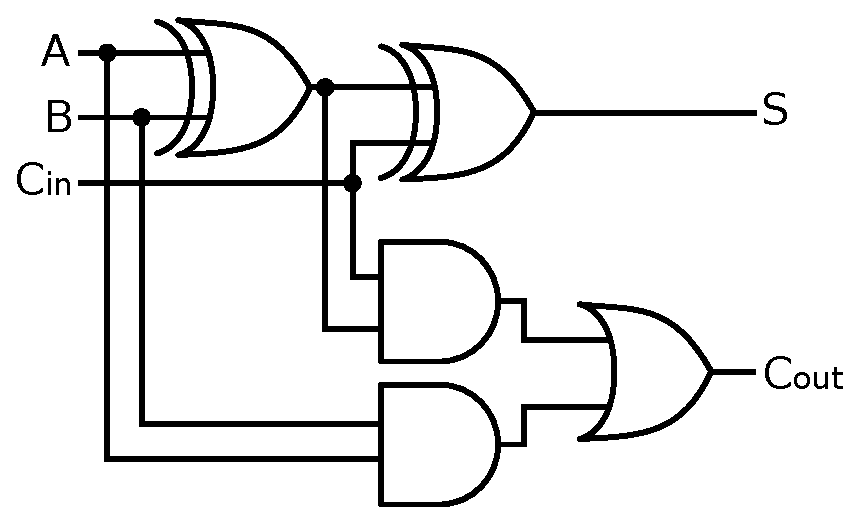
\includegraphics[scale=.4]{img/full-adder.eps}
	\caption{Full adder circuit}
	\label{fig:full_adder_circuit}
\end{figure}

A motivation for the synchronous composition can be found in the following example: a digital design consists of two 1 bit full adders working as separate units. Let $i \in \{1,2\}$ be the index of each adder and $a$ and $b$ the 1 bit entries to be added, $c\_in_i$ the incoming carry signal from another module, $s_i$ the output that represents the lower bit of the sum and $c_i$ the upper bit or carry out, then each 1 bit full adder can be modeled as a single state CLTS.  The FSP syntax would be the following:

\renewcommand{\ttdefault}{pcr}
\begin{figure}[H]
	\begin{lstlisting}[escapeinside={[*}{*]},basicstyle=\scriptsize\ttfamily,columns=flexible,mathescape=true,xleftmargin=3.0ex,keywordstyle=\textbf,morekeywords={if,while,do,else,fork,int,null, algorithm, is, input, output, return, for}]
	FULL_ADDER[i] = (<a[i],s[i]> -> FULL_ADDER[i] | <b[i],s[i]> -> FULL_ADDER[i] 
	| <c_in[i],s[i]> -> FULL_ADDER [i] | <a[i],b[i],c[i]> -> FULL_ADDER[i]
	| <a[i],c_in[i],c[i]> -> FULL_ADDER[i] | <b[i],c_in[i],c[i]> -> FULL_ADDER[i]
	| <a[i],b[i],c_in[i],s[i],c[i]> -> FULL_ADDER[i]| <> -> FULL_ADDER[i]).
\end{lstlisting}
%\caption{Game Structure to CLTS translation algorithm}
\label{fig:full_adder_fsp}
%%\vspace*{-4mm}
\MediumPicture
\end{figure}	

Applying asynchronous composition over single element labeled CLTS models ($FULL\_ADDER[1]$ $\parallel_{a}$ $FULL\_ADDER[2]$), would not properly capture the concurrent occurrence of signals, since it will not allow $<a_1,s_1,a_2,s_2>$ to happen.  

On the other hand, suppose that we are modeling the interaction of three processes $P_1$, $P_2$ and $receiver$ through a common buffer, $P_1$ produces either $a$ or $c$ and
$P_2$ produces either $d$ or $e$. $receiver$ will output a $x$ for each $a$ and a $y$ for each $d$. The FSP syntax would be the following:

\renewcommand{\ttdefault}{pcr}
\begin{figure}[H]
	\begin{lstlisting}[escapeinside={[*}{*]},basicstyle=\scriptsize\ttfamily,columns=flexible,mathescape=true,xleftmargin=3.0ex,keywordstyle=\textbf,morekeywords={if,while,do,else,fork,int,null, algorithm, is, input, output, return, for}]
	P_1 = (a->P_1 | c->P_1).
	P_2 = (d->P_2 | e->P_2).
	Receiver = (<a,x> -> Receiver | <d,y> -> Receiver | c -> Receiver | e -> Receiver).
	\end{lstlisting}
	%\caption{Game Structure to CLTS translation algorithm}
	\label{fig:receiver_fsp}
	%%\vspace*{-4mm}
	\MediumPicture
\end{figure}

Special attention is required when applying the parallel composition operator in order to recreate the system overall interaction. If synchronous semantic ($P_1\parallel_s P_2 \parallel_s receiver$) is to be applied then $receiver$ will not be able to synchronize with both $P_1$ and $P_2$ since at least one action on each component needs to be exercised. In this case, asynchronous composition ($P_1\parallel_a P_2 \parallel_a receiver$)will properly recreate the serialization of events coming from $P_1$ and $P_2$ through the buffer.

Composition semantics should be applied according the each domain, be aware that composition is not commutative if different semantics are applied for the same specification.

%Concurrent semantic $A ||_c B$ (Figure~\ref{fig:concurrent_composition}) captures the behavioral superset of the latter two. It can be used when composing two processes that may not share an implicit synchronizing event, as in the synchronous semantic, but can be observed by a third component that over samples the other two, allowing for the possibility of both concurrent an independent occurrence when observed as a composed system. A synthetic example is shown in Figure~\ref{fig:concurrent_systems}, motivation for this semantic can be found in clock domain crossing examples and micro architecture buffers.
%
%\begin{figure}[bt]
	\centering
	%\SmallPicture
	%\ShowFrame
		\begin{VCPicture}{(-3,-3)(3,2.5)}
			\SetStateLabelScale{1}
			\SetEdgeLabelScale{1}
			\State[1_a]{(-3,1.5)}{A}
			\State[1_b]{(-3,-1.5)}{B}			
			\State[1_c]{(2.5,0)}{C}						
			\Initial[n]{A}
			\Initial[n]{B}
			\Initial[w]{C}						
			%\ChgEdgeLineStyle{dashed} %\EdgeLineDouble
			%\ChgEdgeLineWidth{1.5}
			%\EdgeL{1}{2}{req}
			%\ArcR[.3]{6}{1}{reset}        
			\CLoopSW[.5]{A}{data_a}        
			%\CLoopSE[.5]{A}{idle_a}
			\CLoopSW[.5]{B}{data_b}        
			%\CLoopSE[.5]{B}{idle_b}				
			%\CLoopSW[.5]{C}{idle_c}        
			\CLoopSE[.5]{C}{data_b}					
			\CLoopNW[.5]{C}{data_a}					
			\CLoopNE[.5]{C}{<data_a,data_b,goal>}					
			%\RstEdgeLineWidth{1}
			%\RstEdgeLineStyle %\EdgeLineSimple
			%\EdgeL{2}{3}{grant}
			%\EdgeL[.75]{2}{5}{\overline{grant}}
			%\VArcR{arcangle=-20}{3}{6}{timeout}
			%\ArcR[.6]{3}{6}{timeout}
			%\ArcL{5}{1}{hready}
			%\VArcR{arcangle=-30}{3}{4}{hready}
		\end{VCPicture}

	\caption{A, B and C systems}
	\label{fig:concurrent_systems}
	%%\vspace*{-4mm}
	\MediumPicture
\end{figure}
\begin{figure}[bt]
	\centering
\minipage{0.32\textwidth}	
\centering
	%\SmallPicture
	%\ShowFrame
	\begin{VCPicture}{(-1.5,-1.5)(1.5,1.5)}
		\SetStateLabelScale{.8}
		\SetEdgeLabelScale{1}
		\State[1_{a\parallel_a b}]{(0,0)}{C}
		\Initial[n]{C}
		%\ChgEdgeLineStyle{dashed} %\EdgeLineDouble
		%\ChgEdgeLineWidth{1.5}
		%\EdgeL{1}{2}{req}
		%\ArcR[.3]{6}{1}{reset}        
		\CLoopSW[.5]{C}{data_a}        
		\CLoopSE[.5]{C}{data_b}					
		%\RstEdgeLineWidth{1}
		%\RstEdgeLineStyle %\EdgeLineSimple
		%\EdgeL{2}{3}{grant}
		%\EdgeL[.75]{2}{5}{\overline{grant}}
		%\VArcR{arcangle=-20}{3}{6}{timeout}
		%\ArcR[.6]{3}{6}{timeout}
		%\ArcL{5}{1}{hready}
		%\VArcR{arcangle=-30}{3}{4}{hready}
	\end{VCPicture}
	\caption{A $\parallel_a$ B}
	\label{fig:asynchronous_composition}
\endminipage\hfill
\minipage{0.32\textwidth}%
\centering
	%%\vspace*{-4mm}
	%\SmallPicture
	%\ShowFrame
	\begin{VCPicture}{(-1.5,-1.5)(1.5,1.5)}
		\SetStateLabelScale{.8}
		\SetEdgeLabelScale{1}
		\State[1_{a \parallel_s b}]{(0,0)}{C}
		\Initial[n]{C}
		%\ChgEdgeLineStyle{dashed} %\EdgeLineDouble
		%\ChgEdgeLineWidth{1.5}
		%\EdgeL{1}{2}{req}
		%\ArcR[.3]{6}{1}{reset}        
		\CLoopS[.5]{C}{<data_a, data_b>}        
		%\RstEdgeLineWidth{1}
		%\RstEdgeLineStyle %\EdgeLineSimple
		%\EdgeL{2}{3}{grant}
		%\EdgeL[.75]{2}{5}{\overline{grant}}
		%\VArcR{arcangle=-20}{3}{6}{timeout}
		%\ArcR[.6]{3}{6}{timeout}
		%\ArcL{5}{1}{hready}
		%\VArcR{arcangle=-30}{3}{4}{hready}
	\end{VCPicture}
	\caption{A $\parallel_s$ B}
	\label{fig:synchronous_composition}
\endminipage\hfill
\minipage{0.32\textwidth}%	
\centering
	%%\vspace*{-4mm}
	%\SmallPicture
	%\ShowFrame
	\begin{VCPicture}{(-1.5,-1.5)(1.5,1.5)}
		\SetStateLabelScale{.8}
		\SetEdgeLabelScale{1}
		\State[1_{a\parallel_c b}]{(0,0)}{C}
		\Initial[n]{C}
		%\ChgEdgeLineStyle{dashed} %\EdgeLineDouble
		%\ChgEdgeLineWidth{1.5}
		%\EdgeL{1}{2}{req}
		%\ArcR[.3]{6}{1}{reset}        
		\CLoopSW[.5]{C}{data_a}        
		\CLoopSE[.5]{C}{data_b}					
		\CLoopNE[.5]{C}{<data_a, data_b>}					
		%\RstEdgeLineWidth{1}
		%\RstEdgeLineStyle %\EdgeLineSimple
		%\EdgeL{2}{3}{grant}
		%\EdgeL[.75]{2}{5}{\overline{grant}}
		%\VArcR{arcangle=-20}{3}{6}{timeout}
		%\ArcR[.6]{3}{6}{timeout}
		%\ArcL{5}{1}{hready}
		%\VArcR{arcangle=-30}{3}{4}{hready}
	\end{VCPicture}
	\caption{A $\parallel_c$ B}
	\label{fig:concurrent_composition}
\endminipage\hfill	
	%%\vspace*{-4mm}
\end{figure}
%\begin{figure}[bt]
%\centering
%\SmallPicture
%%\ShowFrame
%\VCDraw{
%    \begin{VCPicture}{(-4,-1.5)(4,2.3)}
%        \SetEdgeLabelScale{1.4}
%        \State[1]{(-3,0)}{1}
%        \State[2]{(0,0)}{2}
%        \State[3]{(3,1)}{3}
%        \State[4]{(-0.5,3)}{4}
%        \State[6]{(0,1.5)}{6}        
%        \State[5]{(3,-1)}{5}
%		\Initial[w]{1}
%        \ChgEdgeLineStyle{dashed} %\EdgeLineDouble
%        %\ChgEdgeLineWidth{1.5}
%        \EdgeL{1}{2}{req}
%        \ArcR[.3]{6}{1}{reset}        
%        \VArcR{arcangle=-30}{4}{1}{process}        
%        %\RstEdgeLineWidth{1}
%        \RstEdgeLineStyle %\EdgeLineSimple
%        \EdgeL{2}{3}{grant}
%        \EdgeL[.75]{2}{5}{\overline{grant}}
%        %\VArcR{arcangle=-20}{3}{6}{timeout}
%        \ArcR[.6]{3}{6}{timeout}
%        \ArcL{5}{1}{hready}
%        \VArcR{arcangle=-30}{3}{4}{hready}
%    \end{VCPicture}
%}
%\caption{Bus Access example ($E$)}
%\label{fig:req_grant}
%%%\vspace*{-4mm}
%\MediumPicture
%\end{figure}
%\begin{figure}[bt]
%\centering
%\SmallPicture
%%\ShowFrame
%\VCDraw{
%    \begin{VCPicture}{(-4,-1.5)(4,2)}
%        \SetEdgeLabelScale{1.4}
%        \State[1]{(-3,0)}{1}
%        \State[2]{(0,-1)}{2}
%        \State[3]{(3,0)}{3}
%        \State[6]{(0,1)}{6}        
%		\Initial[w]{1}
%        \ChgEdgeLineStyle{dashed} %\EdgeLineDouble
%        %\ChgEdgeLineWidth{1.5}
%        \ArcR{1}{2}{req}
%        \ArcR{6}{1}{reset}        
%        %\RstEdgeLineWidth{1}
%        \RstEdgeLineStyle %\EdgeLineSimple
%        \ArcR{2}{3}{grant}
%        %\VArcR{arcangle=-20}{3}{6}{timeout}
%        \ArcR{3}{6}{timeout}
%    \end{VCPicture}
%}
%\caption{Minimized Bus Access ($E_1$)}
%\label{fig:req_grant_sub_1}
%%\vspace*{-4mm}
%\MediumPicture
%\end{figure}
%\begin{figure}[bt]
%\centering
%\SmallPicture
%%\ShowFrame
%\VCDraw{
%    \begin{VCPicture}{(-4,-1.5)(4,2)}
%        \SetEdgeLabelScale{1.4}
%        \State[1]{(-3,0)}{1}
%        \State[2]{(0,0)}{2}
%        \State[3]{(3,1)}{3}
%        \State[6]{(0,1.5)}{6}        
%        \State[5]{(3,-1)}{5}
%		\Initial[w]{1}
%        \ChgEdgeLineStyle{dashed} %\EdgeLineDouble
%        %\ChgEdgeLineWidth{1.5}
%        \EdgeL{1}{2}{req}
%        \ArcR[.3]{6}{1}{reset}        
%        %\RstEdgeLineWidth{1}
%        \RstEdgeLineStyle %\EdgeLineSimple
%        \EdgeL{2}{3}{grant}
%        \EdgeL[.75]{2}{5}{\overline{grant}}
%        %\VArcR{arcangle=-20}{3}{6}{timeout}
%        \ArcR[.7]{3}{6}{timeout}
%        \ArcL{5}{1}{hready}
%    \end{VCPicture}
%}
%\caption{Minimized Bus Access ($E_2$)}
%\label{fig:req_grant_sub_2}
%%\vspace*{-4mm}
%\MediumPicture
%\end{figure}

%\begin{definition} 
%	\label{def:concurrent_composition}(\emph{Concurrent Composition})	Let \automaton{M},\automaton{N}, with $\Delta_M : S_M \times \mathcal{P}(\Sigma_M) \times S_M$, be two CLTS instances, then CLTS concurrent parallel composition is defined as \ltsComposition{M}{N}{c} where $\Delta$ is the smallest relation s.t:
%	\begin{center}
%		\begin{equation}
%		\AxiomC{$(s, l_M, s') \in \Sigma_M,(t, l_N, t') \in \Sigma_N  $}\RightLabel{$l_M \cap \Sigma_N = l_N \cap \Sigma_M$}
%		\UnaryInfC{$((s,t),l_M \cup l_N,(s',t')) \in \Delta$}
%		\DisplayProof
%		\end{equation}	
%		\begin{equation}
%		\AxiomC{$(s, l_M, s') \in \Sigma_M $}\RightLabel{$l_M \cap \Sigma_N = \emptyset$}
%		\UnaryInfC{$((s,t),l_M,(s',t))$}
%		\DisplayProof
%		\quad\quad
%		\AxiomC{$(t, l_N, t') \in \Sigma_N $}\RightLabel{$l_N \cap \Sigma_M = \emptyset$}
%		\UnaryInfC{$((s,t),l_N,(s,t'))$}
%		\DisplayProof
%		\end{equation}
%	\end{center}
%\end{definition}

In the scope of this work asynchronous composition will only be applied over CLTS instances whose transitions contain only one action per label. Asynchronous semantics follow the same rules as in the LTS case.

%\begin{definition} 
%	\label{def:asynchronous_composition}(\emph{Asynchronous Composition}) Let \automaton{M},\automaton{N}, with $\Delta_M : S_M \times \mathcal{P}(\Sigma_M) \times S_M$, be two CLTS instances, then CLTS asynchronous parallel composition is defined as \ltsComposition{M}{N}{a} where $\Delta$ is the smallest relation s.t:
%	\begin{center}
%		\begin{equation}
%		\AxiomC{$(s, l_M, s') \in \Sigma_M,(t, l_N, t') \in \Sigma_N  $}\RightLabel{$l_M \cap \Sigma_N = l_N \cap \Sigma_M \neq \emptyset$}
%		\UnaryInfC{$((s,t),l_M \cup l_N,(s',t')) \in \Delta$}
%		\DisplayProof
%		\end{equation}	
%		\begin{equation}
%		\AxiomC{$(s, l_M, s') \in \Sigma_M $}\RightLabel{$l_M \cap \Sigma_N = \emptyset$}
%		\UnaryInfC{$((s,t),l_M,(s',t))$}
%		\DisplayProof
%		\quad\quad
%		\AxiomC{$(t, l_N, t') \in \Sigma_N $}\RightLabel{$l_N \cap \Sigma_M = \emptyset$}
%		\UnaryInfC{$((s,t),l_N,(s,t'))$}
%		\DisplayProof
%		\end{equation}
%	\end{center}
%\end{definition}

\begin{definition} 
	\label{def:synchronous_composition}(\emph{Synchronous Composition}) Let \automaton{M},\automaton{N}, with $\Delta_M : S_M \times \mathcal{P}(\Sigma_M) \times S_M$, be two CLTS instances, then CLTS synchronous parallel composition is defined as \ltsComposition{M}{N}{s} where $\Delta$ is the smallest relation s.t:
	\begin{center}
		\begin{equation}
		\AxiomC{$(s, l_M, s') \in \Sigma_M,(t, l_N, t') \in \Sigma_N  $}\RightLabel{$l_M \cap \Sigma_N = l_N \cap \Sigma_M$}
		\UnaryInfC{$((s,t),l_M \cup l_N,(s',t')) \in \Delta$}
		\DisplayProof
		\end{equation}	
	\end{center}
\end{definition}

%\begin{definition} 
%	Let $M_1 \ldots M_N$ be CLTS instances s.t. $M_i= (S_{i}, \Sigma_{i}, \Delta_{i}, s_{0}^{i})$ with $\Delta_i : S_i \times l \subseteq \Sigma_i \times S_i$, the concurrent parallel composition \ltsComposition{}{M_i}{} where $\Delta_i$ is the smallest relation s.t:
%	\begin{center}
%		\begin{equation}
%		\AxiomC{$\forall i,j \in 1 \ldots N, i \neq j: ((s_i, l_i, t_i) \in \Delta_i \wedge \forall a \in l_i : a \in (\Sigma_i \cap \Sigma_j) \rightarrow (a \in l_i \wedge a \in l_j)) \vee (l_i = \emptyset \wedge t_i = s_i)$}
%		\UnaryInfC{$((s_1 \ldots s_N),\cup_{i=1}^{N}l_i,(t_1 \ldots t_N)) \in \Delta$}
%		\DisplayProof
%		\end{equation}		
%	\end{center}
%\end{definition}

%\begin{figure}[ht]
%	\begin{center}
%		\renewcommand{\ttdefault}{pcr}
\begin{lstlisting}[escapeinside={[*}{*]},basicstyle=\scriptsize\ttfamily,columns=flexible,frame=lines,mathescape=true,xleftmargin=3.0ex,keywordstyle=\textbf,morekeywords={if,while,do,else,fork,int,null, algorithm, is, input, output, return},numbers=left,numberstyle=\scriptsize]
algorithm compose_automata is
	input: $A_1 \ldots A_N$  the set of CLTS automata to be composed
	input: $type$ an element of $\{synch,asynch,concurrent\}$ the type of composition to be applied
	output: $A$ the CLTS automaton that results from applying $\parallel_{type}$ to $A$
	$s_0$ = $(s^1_{0},\ldots,s^N_{0})$
	$frontier$ = [$s_0$]
	$A$ = create_automaton($s_0$)
	$visited$ = $[]$
	while(|$frontier$| > 0)
		$\Delta_{union}$ = $\emptyset$
		$\Sigma_{union}$ = $\emptyset$		
		
		$s$ = $frontier$.pop()
		$visited$.push($s$)
		for $s_i \in s$ 
			if $\Delta_{union} = \emptyset$
				$\Delta_{union}$ = $\Delta_i(s)$
			else if $\Delta_i(s) \cap \Sigma_{union} = \emptyset$		
				if $type$ = $asynch$
					$\Delta_{union}$ = $\Delta_{union} \cup \Delta_i(s)$
				else
					$\Delta_{union}$ = $\Delta$_cross_product($\Delta_{union}$, $\Delta_i(s)$, $type$)
			else
				$\Delta_{union}$ = $\Delta$_partial_composition($\Delta_{union}$, $\Delta_i(s)$, $\Sigma_{union}$)
		$\Sigma_{union}$ = $\Sigma_{union} \cup \Sigma_i$
		$\Delta$_expand_frontier($frontier$,$\Delta_{union}$, $visited$)				
		add_transitions($A$, $\Delta_{partial}$)
	return $A$

algorithm $\Delta$_cross_product is
	input: $\Delta$ the composite set of transitions already computed for a given state
	input: $\Delta_{i}(s)$ the local set of transitions for a given state $s$ at automaton $A_i$
	input: $type$ an element of $\{synch,asynch,concurrent\}$ the type of composition to	
	output: $\Delta'$ the cross product of the computed set $\Delta$ with $\Delta_{i}(s)$
	$\Delta'$ = $\emptyset$
	for $d \in \Delta$
		for $d' \in \Delta_{i}(s)$
			$\Delta'$ = $\Delta' \cup$ {$s(d)$,($label(d) \cup label(d')$,($t(d)_1, \ldots, t(d')_i, \ldots, t(d)_N$))}
	if $type \neq synch$
		return $\Delta \cup \Delta' \cup \Delta_{i}(s)$
	else
		return $\Delta'$
	
algorithm $\Delta$_partial_composition is
	input: $\Delta$ the composite set of transitions already computed for a given state
	input: $\Delta_{i}(s)$ the local set of transitions for a given state $s$ at automaton $A_i$
	input: $\Sigma$ the composite set of labels already computed for a given state		
	output: $\Delta'$ the partial composition of the computed set $\Delta$ with $\Delta_{i}$ according to $type$
	$\Delta'$ = $\emptyset$
	for $d \in \Delta$
		for $d' \in \Delta_{i}(s)$
			if $\Sigma \cap label(d') = \Sigma_i \cap label(d)$
				$\Delta'$ = $\Delta' \cup$ {$s(d)$,($label(d) \cup label(d')$,($t(d)_1, \ldots, t(d')_i, \ldots, t(d)_N$))}
	return $\Delta'$
				

\end{lstlisting} 
%		\caption{Concurrent Composition Algorithm}
%		\label{fig:dfs-code}
%	\end{center}
%\end{figure}
An algorithm to apply parallel composition over a set of automata (according to a set of semantic definitions) is now presented.  The idea is to start with the composition of the initial states $(s_{0_1},\ldots,s_{0_n})$ as the only element if the $frontier$ to be explored. In subsequent iterations elements are removed and their composed transitions filtered and merged. The resulting target $(s'_1,\ldots,s'_n)$ states are pushed back to the $frontier$ for further evaluation. At every step in the exploration of a particular state $s:(s_1,\ldots,s_n)$ the cross product of the elements of the sets of outgoing transitions $\Delta_1(s_1) \times \ldots \Delta_n(s_n)$ is tested for consistency with respect to the  semantic $(type_1,\ldots,type_{n-1})$. Combinations of source transitions $\delta:(\delta_1,\ldots,\delta_n)$ are iterated depth first obtaining combination $(\delta_1,\ldots,\delta_n)$, then a linear pass over its components merges previous labels (if needed) and checks the partial resulting label $l_{1\ldots i}$  against the following properties:
\[\neg blocks(\delta_{1\ldots i})= \neg(l_{1\ldots i}\cap \Sigma_{i+1} \neq l_{i+1} \cap \Sigma_{1\ldots i}) \]
\[asynch(\delta_{1\ldots i})= \neg (l_{1\ldots i}\cap \Sigma_{i+1} = l_{i+1} \cap \Sigma_{1\ldots i}=\emptyset) \]
\[synch(\delta_{1\ldots i})= \neg (l_{1\ldots i}=\emptyset \wedge l_{i+1} =\emptyset) \]
Property $\neg blocks$ should always hold, then $asynch$ and $synch$ need to be satisfied according to $type_i$ (if $type_i \neq concurrent$). As soon as a property is violated the next element $\delta':(\delta'_1,\ldots,\delta'_n)$ is evaluated, if these properties hold up to $n$ then, if $\delta_{i}:(s_i,l_i,t_i)$, transition
$((s_1,\ldots,s_n),l_{1\ldots n},(t_1,\ldots,t_n))$ is added to the composition.


\begin{figure}[ht]
	\begin{center}
		\renewcommand{\ttdefault}{pcr}
\begin{lstlisting}[escapeinside={[*}{*]},basicstyle=\scriptsize\ttfamily,columns=flexible,frame=lines,mathescape=true,xleftmargin=3.0ex,keywordstyle=\textbf,morekeywords={if,while,do,else,fork,int,null, algorithm, is, input, output, return, for},numbers=left,numberstyle=\scriptsize]
algorithm compose_automata is
	input: $A_1 \ldots A_N$  the set of CLTS automata to be composed
	input: $type$ an element of $\{synch,asynch,concurrent\}$ the type of composition to be applied
	output: $A$ the CLTS automaton that results from applying $\parallel_{type}$ to $A_1 \ldots A_N$
	$s_0$ = $(s^1_{0},\ldots,s^N_{0})$
	$frontier$ = [$s_0$]
	$A$ = create_automaton($s_0$)
	$visited$ = $[]$
	while(|$frontier$| > 0)
		$\Delta_{I}$ = $\emptyset$
		$\Delta_{a}$ = $\emptyset$
		$\Sigma_{a}$ = $\emptyset$		
		$s$ = $frontier$.pop()
		if $s \in visited$
			continue
		$visited$.push($s$)
		$\Delta_{I}$ = $\Delta_0(s)$
		for $s_{i > 0} \in s$ 
			for $d:(s,l,t) \in \Delta_{I}$
				for $d':(s',l',t') \in \Delta_{i}(s)$
					if $\Sigma_{a} \cap l' = \Sigma_i \cap l \wedge \Sigma_i \cap l \neq \emptyset $
						$\Delta_{a}$ = $\Delta_{a} \cup$ {($s$,$l \cup l'$,($t_1, \ldots, t\prime_i, \ldots, t_N$))}
					if $\Sigma_{a} \cap l' = \Sigma_i \cap l \wedge \Sigma_i \cap l = \emptyset$
						if $type \neq asynch$
							$\Delta_{a}$ = $\Delta_{a} \cup$ {($s$,$l \cup l'$,($t_1, \ldots, t\prime_i, \ldots, t_N$))}
						if $type \neq synch$							
							$\Delta_{a}$ = $\Delta_{a} \cup$ {$(s$,$l$,($t_1, \ldots, t_N$))} 
								$\cup$ {$(s$,$l'$,($s_1, \ldots, t'_i, \ldots, s_N$))}
					if $l \cap l' = \emptyset \wedge type \neq synch$
						if $\Sigma_a \cap l' = \emptyset $
							$\Delta_{a}$ = $\Delta_{a} \cup$ {$(s$,$l'$,($s_1, \ldots, t'_i, \ldots, s_N$))} 
						if $\wedge \Sigma_i \cap l = \emptyset$
							$\Delta_{a}$ = $\Delta_{a} \cup$ {$(s$,$l$,($t_1, \ldots,  t_N$))} 							
			$\Delta_{I} = \Delta_{a}$						
			$\Delta_{a} = \emptyset$						
			$\Sigma_{a}$ = $\Sigma_{a} \cup \Sigma_i$
		for $d:(s,l,t) \in \Delta_{I}$
			if $t \notin visited \wedge t \notin frontier$ 
				 $frontier$.push($t$)
			add_transition($A$, $d$)			
	return $A$

\end{lstlisting} 
		\caption{Concurrent Composition Algorithm (closer to code version)}
		\label{fig:dfs-code2}
	\end{center}
\end{figure}

\newpage
\subsection{CLTS control problem}
\textcolor{blue}{In this section} we present the background to define the notion of control problem in the CLTS domain.  

\begin{definition}
	\label{def:legal_clts} \emph{(Legality w.r.t. $E$ and $\mathcal{C}$)} 
	Given CLTS $C = \langle S_C, \Sigma$, $\Delta_C$, $s_{C_0}\rangle$ and $E = \langle S_E,\Sigma,$ $\Delta_E,$ $s_{E_0}\rangle$, where $\Sigma$ is partitioned into actions controlled and monitored (non controllable) by $C$ ($\Sigma=\mathcal{C} \; \cup \;\mathcal{U}$), we say that $C$ is a legal CLTS for $E$ if for all $(s_E,s_C) \in E \parallel_* C$ it holds that
	$\Delta_{E}(s_E)\cap \mathcal{P}(\mathcal{C}) \supseteq \Delta_{C}(s_C)\cap \mathcal{P}(\mathcal{C})$ and also that  $\Delta_{E}(s_E)\cap \mathcal{P}(\mathcal{U}) \subseteq \Delta_{C}(s_C)\cap \mathcal{P}(\mathcal{U})$.
\end{definition}

\begin{definition}
	\label{def:mixed_control_problem} \emph{(CLTS Control Problem)} 
	Let $E$ be a a CLTS instance, if $\mathcal{F}$ is a set of fluents over $\Sigma$ and $\varphi$ an LTL formula over $\mathcal{F}$, then $I = \langle E, \mathcal{F}, \varphi \rangle$ constitutes a CLTS control problem. If a solution to $I$ exists, such a solution will be a CLTS $M$, legal w.r.t. $D$, such that, $E \parallel M \models \varphi$.
\end{definition}


\newpage
\subsection{GR(1) specifications over CLTS}
\textcolor{blue}{In the present work} controller synthesis is applied to specifications where the environment behavior is defined by a set of CLTS instances and games structures. The properties to be satisfied by the specification fall into the GR(1) category and are expressed as LTL formulas.

Since the goal $\varphi$ is restricted to GR(1) formulas we will follow what has been done with LTS based specifications in \cite{DBLP:phd/ethos/DIppolito13}. A translation between CLTS control problems and GR(1) games, and one from strategies into CLTS controller are presented, yielding a framework for CLTS GR(1) control problem synthesis. The GR(1) games used here and in in \cite{DBLP:phd/ethos/DIppolito13} are the same.

\begin{definition}\label{def:gr1_clts_control_problem} \emph{(GR(1) CLTS control problem)} 
	Let $I = \langle E, \mathcal{C}, \mathcal{F}, \varphi \rangle$ be a CLTS control problem, $I$ is a GR(1) CLTS control problem if $\varphi$ satisfies: 
	\[\varphi = (\bigwedge_{i=1}^k\square \Diamond \gamma_i \implies \bigwedge_{j=1}^l\square \Diamond \psi_j)\]
	In the previous definition $\gamma_1, \ldots , \gamma_k$, $\psi_1, \ldots , \psi_l$ are propositional LTL formulas over fluents that represent a set of assumptions over the environment and a set of guarantees the system should satisfy.
\end{definition}

\begin{definition}\label{def:clts_to_gr1_translation} \emph{(GR(1) CLTS control problem to GR(1) game translation)} 
For $I = \langle E, \mathcal{C}, \mathcal{F}=\lbrace fl_1, \ldots, fl_{k+l} \rbrace, \varphi \rangle$ a GR(1) CLTS control problem $gr1(I)=G$ is a GR(1) game $G = \langle S_g,$ $\Gamma^-,$ $\Gamma^+,s_{g_0}\varphi \rangle$ where $S_g = S_e \times \mathbb{B}^{k+l}$ is the set of states and for a state $s_g=(s_e,\alpha_1,\ldots,\alpha_{k+l}) \in S_g$ a fluent
$fl_i$ is said to be satisfied at $s_g$ if and only if $\alpha_i$ is true.
$s_{g_0}=(s_0,Init_1,\ldots,Init_{k+l})$ is the initial state and for every $(s,l,s')\in \Delta_e$, $()s_g,(s'_e,\alpha'_1,\ldots,\alpha'_{k+l}))$ is added to $\Gamma^-$ if $l \in \mathcal{P}(\mathcal{U})$ or $\Gamma^+$ if $l \in \mathcal{P}(\mathcal{C})$, $\alpha'_i$ is set as follows:
\[
\alpha'_i = \begin{cases}
\alpha_i & \text{if } l \notin I_{fl_i} \cup T_{fl_i} \\
\top & \text{if } l \in I_{fl_i}\\
\bot & \text{if } l \in T_{fl_i}
\end{cases}
\]
\end{definition}

If the game $G$ constructed when applying $gr1$ on $I$ is realizable, i.e. if there exists a winning strategy for the system that satisfies $\varphi$ over $G$, then such a strategy can be encoded as a pair of functions $\sigma
$ and $u$. Since $G$ is memory dependent the strategy is split into the function $\sigma$ that picks a successor for any given controllable and reachable state  and $u$ that updates the memory in order to keep track of the guarantee that needs to be satisfied next. 

For a pair $(\sigma,u)$, a controller $M$ is constructed, in order to describe how $M$ is built we define when a transition that follows a winning strategy while preserving legality with respect to a an automaton $E$ is possible.

\begin{definition}\label{def:strat_possible_transition} \emph{(Possible transition)} 
	Let $I = \langle E, \mathcal{C}, \mathcal{F}, \varphi \rangle$ be a CLTS control problem and $G = \langle S_g, \Gamma^-,\Gamma^+,s_{g_0}\varphi \rangle$ be the result of $gr1(I)$, for $s_g=(s_e,\alpha_1,\ldots,\alpha_{k+l}) \in S_g$ and $s'_g=(s'_e,\alpha'_1,\ldots,\alpha'_{k+l}) \in S_g$, action $l \in \mathcal{P}(\Sigma_e)$ is said to be possible if the following condition si satisfied:
	\[possible(s_g,l,s'_g):\forall (s_g,s'_g) \in \Gamma^- \cup \Gamma^+: \exists (s_e,l,s'_e) \in \Delta_e \implies \]
	\[ \forall fl_i \in \mathcal{F}: ((l \cap (I_{fl_i} \cup T_{fl_i} = \emptyset)) \vee (I_{fl_i} \subseteq l \wedge \alpha'_i = \top)\vee (T_{fl_i} \subseteq l \wedge \alpha'_i = \bot))\]
\end{definition}

\begin{definition}\label{def:strat_to_clts_translation} \emph{(Winning strategy to CLTS translation)} 
	Let $f=(\sigma,u)$ with $\sigma:\Omega \times S_g \rightarrow 2^{|S_g|}$ and
	$u:\Omega \rightarrow \Omega$ be a winning strategy for $G = \langle S_g, \Gamma^-,\Gamma^+,s_{g_0}\varphi \rangle$, $clts(f)=M$ is a CLTS instance $M=\langle S_m, \Sigma_m, \Delta_m, s_{0_m}\rangle$ where $S_m \subseteq \Omega \times S_g$ is the set of states
	and $\Delta_m \subseteq S_m \times \mathcal{P}(\Sigma_m) \times S_m$ is the minimal transition relation satisfying the following condition:
	\[\forall s'_g \in S_g: (\exists \omega \in \Omega, (s_g,s'_g) \in (\Gamma^- \cup \Gamma^+), l \in \mathcal{P}(\Sigma_e) \wedge possible(s_g,l,s'_g) \implies \] \[(((\omega,s_g),l,(u(\omega),s'_g))\in \Delta_m) \]
\end{definition}

\newpage
\subsection{CLTS to LTS relation}
La idea es que no podemos traducir CLTS a LTS sin meter deadlocks.
Supongamos la existencia de una traducción $lts:CLTS \rightarrow LTS$ que debería cumplir con lo siguiente, si $A=\langle S, \Sigma, \Delta, s_0 \rangle$ es un CLTS y $A'=lts(A)=\langle S', \Sigma', \Delta', s'_0 \rangle$ es su traducción, querríamos que se cumpla que se pueden proyectar los estados del CLTS, que al menos contiene el alfbeto original y que hay caminos consistentes entre los estados proyectados:

\[S \subseteq S', \Sigma \subseteq \Sigma', s_0 = s'_0\]
Para los estados proyectados pedimos que la relación de transición permita reconstruir un camino donde aparezcan los elementos de la etiqueta orginal preservando cardinalidad:
\[ \forall (s,l,s') \in \Delta, \exists s \xRightarrow[]{l} s' \in \Delta': |l'\downarrow_{\Sigma}| = |l| \]
Queremos ver si se cumple la siguiente propiedad:
\[\exists lts: CLTS \rightarrow LTS | \forall A,B:CLTS, lts(A) \parallel lts(B) = lts(A \parallel_s B)\]
Para esto vamos a usar tres CLTSs de referencia:
\[M_1 = \langle \lbrace 1,2 \rbrace, \lbrace a,b,c \rbrace, \lbrace\langle 1, \lbrace a,b \rbrace, 2 \rangle\rbrace, 1 \rangle\]
\[M_2 = \langle \lbrace 1,2 \rbrace, \lbrace b,c \rbrace, \lbrace \langle 1, \lbrace b,c \rbrace, 2 \rangle\rbrace, 1 \rangle\]
\[M_3 = \langle \lbrace 1,2 \rbrace, \lbrace a,b \rbrace, \lbrace \langle 1, \lbrace a,b \rbrace, 2 \rangle\rbrace, 1 \rangle\]

Aplicando la traducción sobre $M_1$ podemos decir que:
\[M'_1 = lts(M_1) \implies ( 1 \xRightarrow[]{l'} 2 \in \Delta_{M'_1} \wedge |l'\downarrow_{\lbrace a,b,c\rbrace}|= |\lbrace a, b \rbrace | )\]
Si este es el caso vale alguna de las dos opciones siguientes:
\[1 \xRightarrow[]{l'} 2: 1 \xRightarrow[]{p}\xrightarrow{a}\xRightarrow[]{p'}\xrightarrow{b}\xRightarrow[]{p''}2\]
\[1 \xRightarrow[]{l'} 2: 1 \xRightarrow[]{r}\xrightarrow{b}\xRightarrow[]{r'}\xrightarrow{a}\xRightarrow[]{r''}2\]
Y para $M_2$:
\[M'_2 = lts(M_2) \implies ( 1 \xRightarrow[]{l''} 2 \in \Delta_{M'_2} \wedge |l''\downarrow_{\lbrace b,c\rbrace}|= |\lbrace b,c \rbrace | )\]
Si este es el caso vale alguna de las dos opciones siguientes:
\[1 \xRightarrow[]{l''} 2: 1 \xRightarrow[]{u}\xrightarrow{b}\xRightarrow[]{u'}\xrightarrow{c}\xRightarrow[]{u''}2\]
\[1 \xRightarrow[]{l''} 2: 1 \xRightarrow[]{v}\xrightarrow{c}\xRightarrow[]{v'}\xrightarrow{b}\xRightarrow[]{v''}2\]
Pero recordando que $M_{\parallel}=M_1 \parallel_s M_2=\langle \lbrace 1 \rbrace, \lbrace a,b,c \rbrace, \emptyset, 1 \rangle$ bloquea, los pares de prefijos entre $p,r$ y $u,v$ debería bloquear, con lo cual, por ej. debería valer $p_1 \in \Sigma_{M'_2}$, $u_1 \in \Sigma_{M'_1}$ y $p_1 \neq u_1$.

\textbf{Suponiendo que la extensión del alfabeto se consigue por combinación de elementos de $\Sigma$} (por ej. concatenación, que si así no fuese no hay cota de finitud para la extensión, porque cualquier autómata que tenga el mismo alfabeto más un elemento $x$ y está compuesto por una única transición $1 \xrightarrow{x} 2$ tendría que bloquear siempre, entonces un elemento particular debería ser agregado para $x$), tendríamos la siguiente situación:

\[lts(M_2 \parallel_s M_3) \neq lts(M_2)\parallel lts(M_3)\]

Porque $lts(M_2)\parallel lts(M_3)$ no puede producir prefijo $abc$ por haber extendido su alfabeto a poteriori ($\Sigma = \lbrace a,b,c \rbrace$)
pero la composición no bloquearía con:

\[M_1 = \langle \lbrace 1,2 \rbrace, \lbrace a,b,c \rbrace, \lbrace\langle 1, \lbrace c \rbrace, 2 \rangle\rbrace, 1 \rangle\]

\newpage
\subsection{CLTS and Game Structures interoperability}
When writing a specification or an abstraction of a digital system it is convenient to describe its behavior with game structures. This formalism captures the semantic of a two player game where the first participant, the environment, observes the state of both input and output variables at a given point of time to define a new valuation for the input, only then the second player, the system, observes both the previous and the current partial states to define the new valuation for the output. 

The set of possible actions for each player is described as relations between current and next (primed) state's variables. Satisfaction of $\gsRhoE: \gsX \times \gsY \times \gsX'$ describes the values that $\gsX'$ can take when $\gsX$ and $\gsY$ are fixed. Both the initial conditions and the transition relations can be described as boolean formulas which in turn can be represented with OBDDs. OBDDs can be composed, restricted over a subset of known values, checked for satisfiability and equality among other operations. Algorithms that work with OBDDs can and do process sets of states at each step, but finite state machines, such as CLTS, can only be processed one state at a time.

\begin{definition}
	\label{def:GS} \emph{(Game Structures)} 
	A \emph{Game Structure} (GS) $G =  \langle \gsV, \gsX, \gsY, \gsTheE, \gsTheS, \gsRhoE, \gsRhoS, \varphi \rangle$ consists of the following:
	\begin{itemize}
		\item $\gsV = \{v_1,\ldots,v_n\}$ : A finite set of typed state variables over finite domains, without loss of generality we assume that they are all Boolean. In the context of a game structure a state is defined as an assignment of $\gsV$, $s \in \Sigma_{\gsV}$.
		\item $\gsX \subseteq \gsV$ is a set of input variables.
		\item $\gsY = \gsV \setminus \gsX$ is a set of output variables.
		\item $\gsTheE$ is an assertion over $\gsX$ characterizing the initial states of the environment.
		\item $\gsTheS$ is an assertion over $\gsV$ characterizing the initial states of the system.		
		\item $\gsRhoE(\gsV,\gsX')$ is the transition relation of the environment, it identifies a valuation $s_{\gsX} \in \Sigma_{\gsX}$ as a possible input in state $s$ if $(s,s_{\gsX}) \models \gsRhoE$.
		\item $\gsRhoS(\gsV,\gsX',\gsY')$ is the transition relation of the system, it identifies a valuation $s_{\gsY} \in \Sigma_{\gsY}$ as a possible output in state $s$ reading input $s_{\gsX} $if $(s,s_{\gsX}, s_{\gsY}) \models \gsRhoS$.		
		\item $\varphi$ is the winning condition, given by an LTL formula.
	\end{itemize} 
\end{definition}

\begin{definition}
	\label{def:GS_play} \emph{(Play over Game Structure)} 
	Let $G =  \langle \gsV, \gsX, \gsY, \gsTheE, \gsTheS, \gsRhoE, \gsRhoS, \varphi \rangle$ be a game structure, $\sigma = \sigma_1,\sigma_2,\ldots \in (2^{\mathcal{V}})^\omega$ is a play over $G$ if the following holds:
	\begin{itemize} 
		\item The initial condition is satisfied, i.e. $\theta_e(\sigma_1|_{\mathcal{X}}) \wedge \theta_s(\sigma_1)$
		\item The valuations are updated according to $\rho$,
		 $\forall i \in 2\ldots: \rho_e(\sigma_{i-1}, \sigma_i|_{\mathcal{X}}) \wedge \rho_s(\sigma_{i-1}, \sigma_i|_{\mathcal{X}},\sigma_i|_{\mathcal{Y}})$		
	\end{itemize}
\end{definition}

A play $\sigma$ satisfies LTL formula $\varphi$  if $\sigma_1 \models \varphi$ according to the following inductive definition:

\begin{tabular}{ l c l }
	$\sigma_i \models_d v$ & $\triangleq$ & $v \in \sigma_i$ for any $v \in \mathcal{V}$\\	
	$\sigma_i \models_d \neg \varphi$ & $\triangleq$ & $\sigma_i \not\models_d \varphi$\\
	$\sigma_i \models_d \varphi \vee \psi$ & $\triangleq$ & $(\sigma_i \models_d \varphi) \vee (\sigma_i \models_d \psi)$\\
	$\sigma_i \models_d \bigcirc \varphi$ & $\triangleq$ & $\sigma_{i+1} \models_d \varphi$\\
	$\sigma_i \models_d \varphi \U \psi$ & $\triangleq$ & $\exists j \geq i . \sigma_j \models_d \psi \wedge \forall i \leq k \le k. \sigma_k \models_d \varphi$\\
\end{tabular}

A game structure $G$ satisfies LTL formula $\varphi$ if it is satisfied by all of its plays.

Many non trivial digital designs require the definition of state machines to some extent or another, while at the same time high level specifications can involve interactions with digital or truly concurrent components. Under these circumstances a mixed specification over both a finite state process algebra and a LTL game structure definition is desirable.  In order to reason about their composed behavior a proper common representation is needed. Our approach is to transform the game structure into its equivalent finite state automaton and then compose both using one of the parallel composition semantics.

\textcolor{blue}{We now present} the background required to relate the model checking approach in game structures to an equivalent control problem in the CLTS domain.  The main idea behind this is that any game structure specified as a set of LTL formulas induces an equivalent automaton. A pair of translations from a set of LTL formulas to a Kripke structure and from a Kripke structure to a CLTS are introduced first and then a direct transformation between a set of LTL formulas and a CLTS structure.

\begin{definition}
	\label{def:Kripke} \emph{(Kripke Structures)} 
	Let $AP$ be a set of atomic propositions, a \emph{Kripke Structure} (KS)  $K$ over $AP$ is a tuple $K =  \langle S, I, R, L \rangle$ consisting of the following:
	\begin{itemize}
		\item $S$ a finite set of states
		\item $I \subseteq$ a set of initial states
		\item $R \subseteq S \times S$ a transition relation
		\item $L: S \rightarrow 2^{AP}$ a labeling function
	\end{itemize} 
\end{definition}

The translation between game structures and Kripke interprets valuations as states, and relations between those as transitions. Let $G$ be the game structure to be translated and $K=\langle S, I, R, L \rangle$ the target Kripke structure over $AP$. 
Assume that $|AP|=|\mathcal{V}|$ and that for each $v_i \in \mathcal{V}$ exists a proposition $\cdot(v_i) \in AP$. Valuations over $AP$ in $G$ are mapped to states in $S$ as follows, given a valuation $v \in \mathcal{V}$, $\cdot(v)$ represents a unique state in $S$ such that  $|L(\cdot(v))| = |v|$ and for each $v_i \in v$ it holds $\cdot(v_i) \in L(\cdot(v))$. The translation starts with $K$ having an initial state $s_0$ with no valuation associated to it. For every $x \in 2^{|X|}$ where $\theta_e(x)$ holds, a new state $\cdot(x)$ and transition $(s_0, \cdot(x))$ are added to $K$, then for each $x \in 2^{|X|}$, $y \in 2^{|Y|}$ such that $\theta_e(x)$ and $\theta_s(x \cup y)$ hold, state $\cdot(x \cup y)$ and transition $(\cdot(x), \cdot(x \cup y)$ are added to $K$.  For every $v,x' \in 2^{|V|\times|X'|}$ satisfying $\rho_e(v,x')$, a new state $\cdot(v \cup x')$ and transition $(\cdot(v), \cdot(v\cup x'))$ are added to $K$, and for each valuation $v,x',y' \in 2^{|V|\times|X'|\times|Y'|}, $ satisfying $\rho_e(v, x')$ and $\rho_s(v,x',y')$, state $\cdot(x \cup y)$ and transition $(\cdot(v \cup x'), \cdot(x \cup y))$ are added to $K$. 
If the Kripke structure is constructed according to the previous translation, the following properties hold, describing the relation between plays over $G$ and paths over $K$:
	\[\begin{aligned}[t]
	\forall x, y: \theta_e(x) \wedge \theta_s(x,y)& \implies\\
	&(s_0, \cdot (x)), (\cdot(x), \cdot (x \cup y)) \in R \\
	&\wedge \forall x_i \in x: \cdot(x_i) \in L(\cdot(x)) \wedge \forall v_i \in x \cup y : \cdot(v_i) \in L(\cdot(x \cup y))\\
	\forall x, y : \exists v \rho_e(v,x) \wedge \rho_s(v,x,y)& \implies\\
	&(\cdot(v), \cdot(v \cup x)), (\cdot(v \cup x),\cdot(x \cup y)) \in R\\
	&\wedge \forall v_i \in v: \cdot(v_i) \in L(\cdot(v)) \\
	&\wedge \forall w_i \in v \cup x: \cdot(w_i) \in L(\cdot(v \cup x))\\
	&\wedge \forall z_i \in x \cup y: \cdot(z_i) \in L(\cdot(x \cup y))	
	\end{aligned}
	\] 

A translation between LTL formulas over atomic propositions in $K$ and boolean variables in $G$ is straight forward, since the only consideration to be taken is regarding the atomic case of formula $\varphi$ (consisting of a single variable $v_i$). Suppose that $\cdot(\varphi)$ is the translation from boolean variables into atomic propositions, we say that $\varphi$ is satisfied in a play $\sigma=s_0s_1\ldots s_i$ over $G$ if $v_i \in s_i$. In our case this also implies that $\cdot(\varphi)$ is satisfied in the path $\rho=\cdot(s_0)\cdot(s_1)\ldots \cdot(s_i)$ over $K$, since $\cdot(v_i)$ appears in $L(\cdot(s_i))$. It follows from this observation, that if $K$ is the Kripke structure constructed from $G$ following the previous translation, then LTL satisfaction is preserved between structures.

The second step of our composed translation is to transform $K$ into a CLTS instance $M$.
The set of states is kept as is and the labels are moved from $L$ in $K$ to $\Delta$ in $M$. If $M=\langle S, \Sigma, \Delta, s_0 \rangle$ is constructed fom $K =\langle S,I,R,L \rangle$ over $AP$, then both state sets are equal, $s_0$ is the only element in $I$, (since it was, in turn, constructed from $G$) and both $\Sigma$ and $\Delta$ are defined as follows:

\[\forall a \in AP: a\uparrow \in \Sigma \wedge a\downarrow \in \Sigma \]
\[\forall (s, s') \in R: (s, \delta(s,s'), s') \in \Delta \]

Where we add labels to the transitions in $\Delta$, indicating the change of individual variables between valuations. If a variable keeps its value then it will not take part in the transition, otherwise if, for instance, variable $v$ is present in $s$ but not in $s'$, the change is made explicit by adding $v\downarrow$ to the concurrent label.

\[\delta(s,s'): \lbrace label(a,s,s') | a \in L(s) \neq a \in L(s') \rbrace\]
\[
label (a,s,s') = \begin{cases}
a\uparrow & \text{if } a \in L(s') \\
a\downarrow & \text{if } a \in L(s)
\end{cases}
\]

Now if $\cdot(\varphi)$ is the translation from atomic propositions into fluents, and a set of fluents $\mathcal{F}$ exists containing, for each proposition $a$ a fluent $\langle a\uparrow, a\downarrow \rangle$, we say that, again observing only the atomic case where the formula consists of a single variable, $\varphi$ is satisfied in a path $\rho=s_0 s_1\ldots s_i$ over $K$ if $v_i$ appears in $L(s_i)$. In our case this also implies that $\cdot(\varphi)$ is satisfied in the path $\pi=\cdot(s_0)\cdot(s_1)\ldots \cdot(s_i)$ over $M$ since, from $v_i \in L(s_i)$ follows that at some point the proposition started appearing in states leading to $s_i$, suppose that $s_j$ was the first state were $v_i$ appeared and was kept until reaching $s_i$ ($\forall j \leq k \leq i: v_i \in L(s_k)$), then transition $(s_{j-1},s_j) \in R$ was translated as $(s_{j-1}, \delta(s_{j-1},s_j),s_j)$ and $v_i\uparrow \in \delta(s_{j-1},s_j)$ since its value changed from one state to the other. It follows from this observation, that if $M$ is the CLTS structure constructed from $K$ following the previous translation, then LTL satisfaction is preserved between structures.

Now we can introduce a direct translation between game structures and CLTS instances.

\begin{definition}
	\label{def:fl_ltl} \emph{(LTL over $\mathcal{V}$ to LTL over $\mathcal{F}$ translation)} 
	Let $\varphi$ be a LTL formula over countable boolean variables $\mathcal{V}$, and if $\mathcal{F}$ is the minimal fluent set containing $v_f = \langle v\uparrow, v\downarrow \rangle$ for each $v \in \mathcal{V}$, $fl(\varphi)$ is an equivalent LTL formula over fluents according to the following inductive definition:\\
	
\begin{tabular}{ l c l }
	$fl(v)$ & $\triangleq$ & $v_f$\\	
	$fl(\neg \varphi)$ & $\triangleq$ & $\neg fl(\varphi)$\\
	$fl(\varphi \vee \psi$ & $\triangleq$ & $fl(\varphi) \vee fl(\psi)$\\
	$fl(\bigcirc \varphi)$ & $\triangleq$ & $\bigcirc fl(\varphi)$\\
	$fl(\varphi \U \psi)$ & $\triangleq$ & $fl(\varphi) \U fl(\psi)$\\
\end{tabular}	
\end{definition}


\begin{definition}
	\label{def:gs_to_clts_translation} \emph{(Game Structure to CLTS translation)} 
Let $G =  \langle \gsV, \gsX, \gsY, \gsTheE, \gsTheS, \gsRhoE, \gsRhoS, \varphi \rangle$ be a game structure, $clts(G)=M$ is a CLTS instance such that $G \models \varphi$ $\iff$ $M \models fl(\varphi)$.
\end{definition}

Let $G$ be the game structure to be translated and $M=\langle S, \Sigma, \Delta, s_0 \rangle$ the target CLTS, i.e. the candidate for $clts(G)$.  The alphabet is defined as the minimal set satisfying 
$\forall v \in \mathcal{V}: v\uparrow \in \Sigma, v\downarrow \in \Sigma$. 
In order to construct $\Delta$ variables will be mapped as following:

\[
\cdot(v_i,v) = \begin{cases}
v_i\uparrow & \text{if } v \in v \\
v_i\downarrow & \text{if } v \not\in v
\end{cases}
\]
\[\cdot(v,v') = \lbrace \cdot (v_i,v') | v_i \in v \neq v_i \in v' \rbrace \]
Suppose that a set of mappings $s:\mathcal{X}\rightarrow S$,$s:\mathcal{V} \rightarrow S$,$s:\mathcal{V} \times \mathcal{X} \rightarrow S$ exist, relating a valuation over those set of variables with a distinct state in the CLTS automaton, then $\Delta$ is the minimal relation satifying:
	\[
	\forall x, y: \theta_e(x) \wedge \theta_s(x,y) \implies \exists s(x),s(x,y) : (s_0, \cdot (\bot, x), s(x)), (s(x), \cdot (x,(x \cup y)), s(x,y)) \in \Delta 
	\] 
	\[
	\forall x, y : \exists v: \rho_e(v,x) \wedge \rho_s(v,x,y) \implies\]
	\[\exists s(v),s(v,x),s(x,y) : (s(v), \cdot (v, v \cup x),s(v,x)), (s(v,x), \cdot (v \cup x,x \cup y), s(x,y)) \in \Delta 
	\] 

As in the previous cases, and showing only the atomic case where the formula consists of a single variable $v$, $\varphi$ is satisfied in move $\sigma_i$ within play $\sigma=\sigma_1,\sigma_2\ldots ,\sigma_i$ on $G$ if $v$ belongs to $\sigma_i$. In our case this also implies that $fl(\varphi)$ is satisfied in state $s_i$ within the path $\pi=s(x),s(x,y),\ldots,s_i=s(\sigma_i)$ over $M$ since, from $v \in \sigma_i$ follows that at some point the proposition started appearing in states leading to $s_i$, suppose that $s_j$ was the first state were $v$ appeared and was kept until reaching $s_i$ ($\forall j \leq k \leq i: v \in \sigma_k$), then step $(\sigma_{j-1},\sigma_j) \in G$ was translated as $(s(\sigma_{j-1}), \cdot(\sigma_{j-1},\sigma_j),\sigma_{j})$ and $v\uparrow \in \cdot(\sigma_{j-1},\sigma_j)$ since its value changed from one state to the other. It follows from this observation, that if $M$ is the CLTS structure constructed from $G$ following the previous translation, then LTL satisfaction is preserved between structures.
%
%\begin{definition}
%	\label{def:mixed_env} \emph{(Mixed Environment Definition)} 
%	A mixed environment $D = \langle E, G \rangle$ is defined over both CTLS instances and game structures as follows,
%	let $E_1,\ldots,E_n$ be a set of CLTS automata and $G_1,\ldots,G_m$ a set of game structures,
%	then each component is defined as $G=\langle \mathcal{V}, \mathcal{X}, \cap_{i \in 1..m}\theta_{e_i}, \cap_{i \in 1..m}\theta_{s_i},$ $\cap_{i \in 1..m}\rho_{e_i},$ $\cap_{i \in 1..m}\rho_{s_i}\rangle$ and $E = \parallel_{*,i \in 1..n} E_i$, where $\parallel_*$ stands for either the asynchronous or synchronous composition semantic.
%	The composed behavior of $D$ is defined by the automaton $E \parallel_* clts(G)$, thus $\langle E, G \rangle \models \varphi$ means $(E \parallel_* clts(G)) \models \varphi$.
%\end{definition}
%
%
%\begin{definition}
%	\label{def:mixed_control_problem} \emph{(Mixed Control Problem)} 
%	Let $D= \langle E, G \rangle$ be a mixed environment, if $\mathcal{F}$ is a set of fluents over $\Sigma$ and $\varphi$ an LTL formula over $\mathcal{F}$, then $I = \langle E, G, \mathcal{F}, \varphi \rangle$ conforms a mixed control problem. If $I$ is consistent and a solution to $I$ exists, such a solution will be a CLTS $M$, legal w.r.t. $D$, such that, $D \parallel M \models \varphi$.
%\end{definition}
%
%\begin{definition}
%	\label{def:consistent_mixed_control_problem} \emph{(Consistent Mixed Control Problem)} 
%	Let $I = \langle E, G, \mathcal{F}, \varphi \rangle$ be a mixed control problem, $I$ is consistent if $\forall v \in \mathcal{V}: v\uparrow, v\downarrow \in \Sigma$, let
%	$\mathcal{Y} = \mathcal{V}\setminus \mathcal{X}$, $v \in \mathcal{Y}$ implies $v\uparrow, v\downarrow \in \mathcal{C}$, $\dot{v} = \lbrace v\uparrow, v\downarrow \rbrace \in \mathcal{F}$ and both $E$ and $clts(G)$ are consistent w.r.t. $\mathcal{F}$.
%\end{definition}


We can now introduce algorithm ~\ref{fig:gs_to_clts_algorithm}, that takes a game structure, represented as a set 
$\gsTheE$, $\gsTheS$, $\gsRhoE$, $\gsRhoS$, $\varphi$ of OBDDs, one for each formula, and produces the CLTS automaton $A$ that preserves its behavior. Since the state space is finite ($2^{|\gsV|}$ at most) and the number of states reached by applying $\gsRhoS(\gsRhoE(v))$ increases monotonically (when starting from $\gsTheS(\gsTheE)$), a least fixed point exists, the algorithm computes such fixed point while progressively creating the transition relation $\Delta$. \texttt{valuations}($\psi$) gives the set of valuations over $\gsV$ for a formula $\psi$ represented with an OBDD. Each valuation induces a unique state in $A$. \texttt{restrict}($\psi$, $s$) fixes a subset of variables in $\psi$ according to $s$ a valuation. If $\varphi$ is the set of propositional formulas involved in the winning condition, \texttt{evaluate\_condition}($A$, $\varphi$, $s$) evaluates the satisfaction of each such formulas according to valuation $s$ and maps the result to $s$ as a state in $A$.
\newpage
\renewcommand{\ttdefault}{pcr}
\begin{figure}[bt]
\begin{lstlisting}[escapeinside={[*}{*]},basicstyle=\scriptsize\ttfamily,columns=flexible,frame=lines,mathescape=true,xleftmargin=3.0ex,keywordstyle=\textbf,morekeywords={if,while,do,else,fork,int,null, algorithm, is, input, output, return, for},numbers=left,numberstyle=\scriptsize]
algorithm gs_to_clts is
	input: $GS$ a set of OBDD structure representing LTL formulas
	output: $A$ a CLTS automaton equivalent to the game structure induced by $GS$
	
	$A$ $\leftarrow$ create_automaton($s_0$)
	$visited \leftarrow \{s_0\}$ 
	$frontier \leftarrow$ valuations($\gsTheE$)
	for $s \in frontier$:
		add_transition($A$, $s_0$, $s$)
		evaluate_condition($A$, $\varphi$, $s$)		
	$new\_frontier \leftarrow $ [] 
	for $s \in frontier$:
		add($visited$,$s$)
		$current \leftarrow$ valuations(restrict($\gsTheS$, $s$))
		for $s' \in current$:
			add_transition($A$, $s$, $s'$)
			evaluate_condition($A$, $\varphi$, $s'$)
			if $s' \not\in new\_frontier$:			
				add($new\_frontier$, $s'$)
	$frontier \leftarrow new\_frontier$
	while $frontier \neq$ []:
		while $frontier \neq$ []:		
			$s_{sys} \leftarrow$ pop($frontier$)
			if $s_{sys} \in frontier$:
				continue
			$current \leftarrow$ valuations(restrict($\gsRhoE$, $s_{sys}$))
			for $s' \in current$:
				add_transition($A$, $s_{sys}$, $s'$)
				evaluate_condition($A$, $\varphi$, $s'$)			
				if $s' \not\in new\_frontier$:			
					add($new\_frontier$, $s'$)				
		$frontier \leftarrow new\_frontier$		
		while $frontier \neq$ []:		
			$s_{env} \leftarrow$ pop($frontier$)
			if $s_{env} \in frontier$:
			continue
			$current \leftarrow$ valuations(restrict($\gsRhoS$, $s_{env}$))
			for $s' \in current$:
				add_transition($A$, $s_{env}$, $s'$)
				evaluate_condition($A$, $\varphi$, $s'$)			
				if $s' \not\in new\_frontier$:			
					add($new\_frontier$, $s'$)				
		$frontier \leftarrow new\_frontier$				
	return $A$
\end{lstlisting}
\caption{Game Structure to CLTS translation algorithm}
\label{fig:gs_to_clts_algorithm}
%%\vspace*{-4mm}
\MediumPicture
\end{figure}


\newpage
\subsection{CLTS equivalence check and minimization}
\textcolor{blue}{CLTS equivalence} is defined in the same way as LTS is. Two instances $E =  (S, \Sigma, \Delta, s_0)$,
$E' =  (S', \Sigma', \Delta', s_0')$ are equivalent if they are bisimilar. This means that they satisfy the same set of CTL* formulas. Given two CLTS instances we propose an algorithm based on \cite{paige1987three}, it yields a partition over the set $S \times S'$ describing the bisimulation relation between $E$ and $E'$.
$B \subseteq S \times S'$ is a bisimulation relation between $E$ and $E'$ if and only if:

\[\begin{aligned}
	\forall s, s' \in S \times S': & B(s,s') \implies \\
	&\forall l,t \text{ s.t. } (s,l,t) \in \Delta  :\exists t' \text{ s.t. } (s',l,t') \in \Delta' \wedge B(t,t')\\
	&\forall l',t' \text{ s.t. } (s',l',t') \in \Delta' :\exists t \text{ s.t. } (s,l',t) \in \Delta \wedge B(t,t')\\	
\end{aligned}\]

The general algorithm is not different to previous partition based approaches, let $E$ and $E'$ be our two structures, we define a sequence of relations$B_0^*,B_1^*,\ldots$ on $S \times S'$ as follows:

\begin{itemize}
	\item $B_0^*(s_0,s_0') \wedge \forall s,s' \in S \times S' \setminus \{s_0,s_0'\}: B_0^*(s,s')$
	\item $\begin{aligned}[t]
	B_{n+1}^*& \iff B_m^*(s,s') \text{ } \wedge\\
		&\forall l,t \text{ s.t. }(s,l,t) \in \Delta \implies \exists t':(s',l,t') \in \Delta' \wedge B_n^*(t,t') \text{ } \wedge\\
		&\forall l',t' \text{ s.t. }(s',l',t') \in \Delta' \implies \exists t:(s,l',t) \in \Delta \wedge B_n^*(t,t')\end{aligned}$
\end{itemize}

Following previous algorithms it suffices to prove that if $B$ is a bisimulation between $E$ and $E'$ then $B$ is contained in $B^* \forall i \geq 0$.  Applying inductive reasoning on $i$, is clear that $B$ is contained in $B_0^*$ since any pair of $B$ are either the initial states, or non initial. Assuming 
$B \subseteq B_n^*$ and $B(s,s')$, if $(s,l,t) \in \Delta$. Because $B$ is bisimulation, there exists $s'$ s.t. $(s',l,t') \in Delta'$ and $B(s,s')$, since $B$ is contained in $B_n^*$ it follows that $B_n^*(t,t')$.
A similar approach holds for the third condition, proving $B_{n+1}^*(s,s')$ which shows that $B^*$ is the largest bisimulation between $E$ and $E'$.

Below two other algorithms are shown, the first minimizes an CLTS according to its equivalent states and the second performs an equivalence check between two automata provided they are deterministic minimal instances.

\begin{figure}[H]
	\begin{center}
		\renewcommand{\ttdefault}{pcr}
\begin{lstlisting}[escapeinside={[*}{*]},basicstyle=\scriptsize\ttfamily,columns=flexible,frame=lines,mathescape=true,xleftmargin=3.0ex,keywordstyle=\textbf,morekeywords={if,while,do,else,fork,int,null, algorithm, is, input, output, return,for},numbers=left,numberstyle=\scriptsize]
algorithm fda_minization_adapted is
	input: $A$  a deterministic CLTS automaton
	output: $P$  a partition of equivalent states
	$P$ = $\{\{s_0\}, S \setminus \{s_0\}\}$
	$W$ = $\{S \setminus \{s_0\}\}$
	while($W \neq \emptyset$)
		$A$ = take_one($W$)
		$W$ = $W \setminus \{A\}$
		for $l \in incoming(A)$
			$X$ = $\Delta_l^{-1}(A)$
			for $Y \in P s.t. X \cap Y = \emptyset \wedge Y \setminus X = \emptyset$
				$P$ = $P \setminus Y$
				$P$ = $P \cup (Y \cap X) \cup (Y \setminus X)$				
				if $Y \in W$
					$W$ = $W \setminus Y$				
					$W$ = $W \cup (Y \cap X) \cup (Y \setminus X)$		
				else if $|Y \cap X| \leq |Y \setminus X|$							
					$W$ = $W \cup (Y \cap X)$						
				else
					$W$ = $W \cup (Y \setminus X)$						
	return $P$
\end{lstlisting} 
		\caption{Minimization algorithm}
		\label{fig:fda-adaptation}
	\end{center}
\end{figure}

\begin{figure}[H]
	\begin{center}
		\renewcommand{\ttdefault}{pcr}
\begin{lstlisting}[escapeinside={[*}{*]},basicstyle=\scriptsize\ttfamily,columns=flexible,frame=lines,mathescape=true,xleftmargin=3.0ex,keywordstyle=\textbf,morekeywords={if,while,do,else,fork,int,null, algorithm, is, input, output, return,for},numbers=left,numberstyle=\scriptsize]
algorithm automata_equivalence is
	input: $A_1$, $A_2$  two deterministic CLTS automata
	output: $true$ if both automata are equivalent, $false$ otherwise
	$frontier$ = [$(s^{1}_0,s^{2}_0)$]
	$visited$ = $[]$
	while(|$frontier$| > 0)
		$(s_1,s_2)$ = $frontier$.pop()
		if $(s_1,s_2) \in visited$
			continue
		$visited$.push($(s_1,s_2)$)
		if($|\Delta_1(s_1)| \neq |\Delta_2(s_2)|$)
			return $false$
		order($\Delta_1(s_1)$)
		order($Delta_2(s_2)$)
		for $i \in [1..|\Delta_1(s_1)|]$
			if label($\Delta_1(s_1)[i]$) $\neq$ label($\Delta_2(s_2)[i]$)
				return $false$
			if (to_state($\Delta_1(s_1)[i]$),to_state($\Delta_2(s_2)[i]$) $\notin visited \cup frontier$
			$frontier$.push((to_state($\Delta_1(s_1)[i]$),to_state($\Delta_2(s_2)[i]$))
	return $true$

\end{lstlisting} 
		\caption{Equivalence check algorithm for deterministic minimal automata}
		\label{fig:equivalence-check}
	\end{center}
\end{figure}

%\begin{figure}[H]
%	\begin{center}
%		\renewcommand{\ttdefault}{pcr}
\begin{lstlisting}[escapeinside={[*}{*]},basicstyle=\scriptsize\ttfamily,columns=flexible,frame=lines,mathescape=true,xleftmargin=3.0ex,keywordstyle=\textbf,morekeywords={if,while,do,else,fork,int,null, algorithm, is, input, output, return,for},numbers=left,numberstyle=\scriptsize]
algorithm automaton_minimization is
	input: $A$  a deterministic CLTS automaton
	output: $A'$  a deterministic minimized CLTS automaton
	hash = initiliaze_$\Delta$_hash($A$)
	do
		changed = $false$
		for $s \in A \wedge$ !changed
			for $t \in \Delta(s) \wedge$ !changed
				for $t'  \in \Delta(s) \wedge t \neq t' \wedge$ !changed
					if hash($t$) = hash($t'$) 
						if $t = t'$
							if $\Delta(s(t)) = \delta(s(t'))$ 
								merge($s(t)$,$s(t')$)
								changed = $true$
		
	while changed = $true$
	return $A$
\end{lstlisting} 
%		\caption{Minimization algorithm}
%		\label{fig:minimization}
%	\end{center}
%\end{figure}


\subsection{CLTS grammar}
\newenvironment{grammar}[2]
{\begin{tabular}{@{}>{$}l<{$}@{\qquad}l@{}}
		\multicolumn{1}{@{}l@{}}{$#1$}&\multicolumn{1}{l@{}}{#2}\\}
	{\end{tabular}}
\begin{figure}[H]
\[
\begin{grammar}{}{}
	D_b \Coloneqq P(x_1=V_1,\ldots,x_k)V_k=B_0 &process definition\\
	\quad D_{l_1},\ldots,D_{l_m}                        & local processes \\
	\quad +\{A_{e_1}, \ldots,A_{e_n} \}                           & alphabet extension \\
	\quad / \{A'_{r_1}\setminus A_{r_1},\ldots, A'_{r_p}\setminus A_{r_p} \} \setminus \{ A_{h_1},\ldots, A_{h_q} \}                         & relabeling and hiding \\
	\\
	D_l \Coloneqq P[x_1^1:L_1^1]\ldots[x_1^n:L_1^n]=B_1, &local process definition\\
	\quad \ldots                        &  \\
	\quad P[x_m^1:L_m^1]\ldots[x_m^n:L_m^n]=B_m &\\
	\\
	B \Coloneqq \text{\textbf{stop}} &deadlock termination\\
	\quad |\quad  \text{\textbf{end}} &normal termination\\
	\quad |\quad  \text{\textbf{error}} &erroneous termination\\
	\quad |\quad  A \rightarrow B_0 &prefixing\\	
	\quad |\quad  P(V_1,\ldots, V_n);B_0 &global process cal\\		
	\quad |\quad  P[V_1]\ldots P[V_n] &local process call\\	
	\quad |\quad  \text{\textbf{if }} V \text{\textbf{ then }} B_1 \text{\textbf{ else }} B_2&conditional branching\\
	\quad |\quad  \text{\textbf{when }} V_1 B_1 | \ldots | \text{\textbf{when }} V_n B_n &choice\\	
	\\
	A \Coloneqq L_1 \ldots L_n &label\\	
	\\
	L \Coloneqq S_0 &action set\\		
	\quad |\quad  V | x:V &expression\\	
	\quad |\quad  \{ A_1, \ldots, A_n \} | x:\{ A_1, \ldots, A_n \} &label set\\	
	\quad |\quad  V_1\ldots V_n | x:V_1\ldots A_n  &range\\		
	\\
	S \Coloneqq act | act, S_0 &action set
\end{grammar}
\]
\label{fig:cfsp_basic_grammar}
\caption{Abstract grammar of the CFSP language: basic processes}
%%\vspace*{-4mm}
\MediumPicture
\end{figure}

\begin{figure}[H]
	\[
	\begin{grammar}{}{}
	D_c \Coloneqq \parallel P(x_1=V_1,\ldots,x_k)V_k=C_0 &process definition\\
	\quad op_p \{A_{p_1},\ldots, A_{p_n} \} \setminus \{ A_{h_1},\ldots, A_{h_q} \}                         & priority and hiding \\
	\\
	op_p \Coloneqq \gg &high priority operator\\
	\quad | \quad \ll    & low priority operator \\	
	\\
	C \Coloneqq P(V_1,\ldots ,V_n) &process call\\
	\quad | \quad C_1 \parallel \ldots \parallel C_n    & asynchronous parallel composition \\		
	\quad | \quad C_1 \parallel_c \ldots \parallel_c C_n    & synchronous parallel composition \\
	\quad | \quad C_0 \setminus \{ A'_1 \setminus A_1, \ldots , A'_n \setminus A_n \}     & relabeling\\	
	\quad | \quad \{ A_1, \ldots , A_n \} : C_0      & labeling\\	
	\quad | \quad \{ A_1, \ldots , A_n \} :: C_0      & sharing\\		
	\quad |\quad  \text{\textbf{if }} V \text{\textbf{ then }} C_1 \text{\textbf{ else }} C_2&conditional\\	
	\quad |\quad  \text{\textbf{forall }} [x_1:L_1]\ldots[x_n:L_n] C_2&replication\\
	 \\				 
	\end{grammar}
	\]
	\label{fig:cfsp_composite_grammar}
	\caption{Abstract grammar of the CFSP language: composite processes}
	%%\vspace*{-4mm}
	\MediumPicture
\end{figure}

\newpage
\bibliographystyle{unsrt}
\bibliography{clts}

\end{document}